\section{Modeling edit distance} \label{sec:apdx:model_distance}
In this section, we describe the details for the three models we used to analyze the edit distance data.

\subsection{Model 1: Edit Distance per Option} \label{sec:apdx:model_distance_option}

\subsubsection{Dependent variables}
The dependent variable for this model is the edit total distance accumulated for an option $D_i$. Distance is a positive continuous variable.

\subsubsection{Independent variables}
The independent variables for this model are the length of the option $L_i$, modeled as a ordinal variable (Equation~\ref{eq:distance_model_1_eta_ordinal}); interface type $I_i$, modeled as a categorical variable; user effect $U_i$ is modeled using a reparameterized approach, where a non-centered parameterization allows for improved sampling efficiency (Equation~\ref{eq:distance_model_1_user_effect}); and the interaction between length and interface type $\phi_{ij}$. Interface and user types were set up with their own hyperpriors. The interaction effect used a non-centered parameterization constrained by an LKJ prior to account for correlations (Equation~\ref{eq:distance_model_1_lkj}). 

\subsubsection{Overall model and Likelihood function}
We modeled the dependent variable using an Exponential distribution (Equation~\ref{eq:distance_model_1}). We expect a long tail of distances across options. The observed outcome variable $D_i$ represents the response for the $i$-th observation parameterized by the latent predictor $\eta_i$. $\eta_i$ is described in Equation~\ref{eq:distance_model_1_eta}.

\begin{align}
    D_i \sim \text{Exponential}(\lambda_i) \label{eq:distance_model_1} \\
    \lambda_i = \exp(\eta_i)\\
    \eta_i = \alpha + \gamma_i + \beta_I[I_i] + \phi_{ij} + U_i \label{eq:distance_model_1_eta} \\
    \gamma_i = \mu_L + \beta_L \cdot L_i \label{eq:distance_model_1_eta_ordinal} \\
    \phi_{ij} = L_{\Omega} \cdot (\sigma_{\phi} \odot z_{\phi}) \label{eq:distance_model_1_lkj} \\
    U_i = \mu_U + \sigma_U \cdot z_U \label{eq:distance_model_1_user_effect}
\end{align}

Priors are defined as:
\begin{align}
    \mu_L, \mu_I, \mu_U, \beta_L, \beta_I, z_{\phi}, z_U &\sim \mathcal{N}(0, 1) \label{eq:priors_global_mean} \\
    \sigma_{\phi} \sim \text{HalfNormal}(0.5) \label{eq:priors_sigma_phi} \\
    \sigma_U \sim \text{Exponential}(0.5) \label{eq:priors_sigma_U} \\
    L_{\Omega} \sim \text{LKJ}(3) \label{eq:priors_L_Omega}
\end{align}

\subsection{Model 2: Edit Distance with Separate Mean and Variance Predictors} \label{sec:apdx:model_distance_variance}

\subsubsection{Dependent Variables}
The dependent variable for this model is the edit distance and its direction \( D_i \). Edit distance in this model is a real number.

\subsubsection{Independent Variables}
The independent variables for this model are:
\begin{itemize}
    \item \textbf{Length of the option (\( L_i \))}: Modeled as an ordinal variable.
    \item \textbf{Interface type (\( I_i \))}: Modeled as a categorical variable.
    \item \textbf{User effect (\( U_i \))}: Modeled using a reparameterized approach for improved sampling efficiency.
    \item \textbf{Interaction between length and interface type (\( \phi_{ij} \))}: Modeled with a non-centered parameterization and constrained by an LKJ prior to account for correlations.
\end{itemize}
Interface and user types were set up with their own hyperpriors.

\subsubsection{Overall Model and Likelihood Function}
We modeled the dependent variable using a Normal distribution with separate predictors for the mean and variance (Equation~\ref{eq:distance_model_2_likelihood}). The reason behind this apprach is to capture the effect of these independent variables to both mean and variance. The observed outcome variable \( D_i \) represents the response for the \( i \)-th observation parameterized by the latent predictors \( \mu_i \) and \( \sigma_{\text{obs},i} \). \( \mu_i \) and \( \sigma_{\text{obs},i} \) are described in Equations~\ref{eq:distance_model_2_mu} and \ref{eq:distance_model_2_sigma}, respectively.

\begin{align}
    D_i &\sim \text{Normal}(\mu_i, \sigma_{\text{obs},i}) \label{eq:distance_model_2_likelihood} \\
    \mu_i &= \alpha_{\mu} + \gamma_{\mu,i} + \beta_{I,\mu}[I_i] + \phi_{\mu,ij} + U_{\mu,i} \label{eq:distance_model_2_mu} \\
    \gamma_{\mu,i} &= \mu_{L,\mu} + \beta_{L,\mu} \cdot L_i \label{eq:distance_model_2_gamma_mu} \\
    % \beta_{I,\mu}[I_i] &= \mu_{I,\mu} + \sigma_{I,\mu} \cdot \text{InterfaceEffect}_{\mu,I_i} \label{eq:distance_model_2_beta_I_mu} \\
    \phi_{\mu,ij} &= L_{\Omega,\mu} \cdot (\sigma_{\phi,\mu} \odot z_{\phi,\mu}) \label{eq:distance_model_2_phi_mu} \\
    U_{\mu,i} &= \mu_{U,\mu} + \sigma_{U,\mu} \cdot z_{U,\mu,i} \label{eq:distance_model_2_user_mu} \\
    \log(\sigma_{\text{obs},i}) &= \alpha_{\sigma} + \gamma_{\sigma,i} + \beta_{I,\sigma}[I_i] + \phi_{\sigma,ij} + U_{\sigma,i} \label{eq:distance_model_2_sigma} \\
    \gamma_{\sigma,i} &= \mu_{L,\sigma} + \beta_{L,\sigma} \cdot L_i \label{eq:distance_model_2_gamma_sigma} \\
    % \beta_{I,\sigma}[I_i] &= \mu_{I,\sigma} + \sigma_{I,\sigma} \cdot \text{InterfaceEffect}_{\sigma,I_i} \label{eq:distance_model_2_beta_I_sigma} \\
    \phi_{\sigma,ij} &= L_{\Omega,\sigma} \cdot (\sigma_{\phi,\sigma} \odot z_{\phi,\sigma}) \label{eq:distance_model_2_phi_sigma} \\
    U_{\sigma,i} &= \mu_{U,\sigma} + \sigma_{U,\sigma} \cdot z_{U,\sigma,i} \label{eq:distance_model_2_user_sigma}
\end{align}

\subsubsection{Priors}
Priors are defined as:
\begin{align}
    \mu_{L,\mu}, \mu_{I,\mu}, \mu_{U,\mu}, \beta_{L,\mu}, \beta_{I,\mu}, z_{\phi,\mu}, z_{U,\mu,i} &\sim \mathcal{N}(0, 1) \label{eq:priors_distance_model_2_mean} \\
    \mu_{L,\sigma}, \mu_{I,\sigma}, \mu_{U,\sigma}, \beta_{L,\sigma}, \beta_{I,\sigma}, z_{\phi,\sigma}, z_{U,\sigma,i} &\sim \mathcal{N}(0, 1) \label{eq:priors_distance_model_2_variance} \\
    \sigma_{\phi,\mu}, \sigma_{\phi,\sigma} &\sim \text{HalfNormal}(0.5) \label{eq:priors_sigma_phi_distance_model_2} \\
    \sigma_{U,\mu}, \sigma_{U,\sigma} &\sim \text{Exponential}(0.5) \label{eq:priors_sigma_U_distance_model_2} \\
    L_{\Omega,\mu}, L_{\Omega,\sigma} &\sim \text{LKJ}(3) \label{eq:priors_L_Omega_distance_model_2}
\end{align}

\subsubsection{Model Results}
Here we provide all pairwise comparisons for the variance which the main text only provided the comparison within the same survey length. Figure~\ref{fig:bayesian_distance_variance} shows the pairwise comparison of the variance of edit distance in the first row followed by the effect size in the second row. An notable result that we omit from the main text is that if we compare the variance between the long and short text, and the variance between the long and short two-phase, we see that the text group had three times the standard deviation compared to the two-phase group. This indicates that the organization phase minimize the added length of the survey.

\begin{figure}[h!]
    \centering
    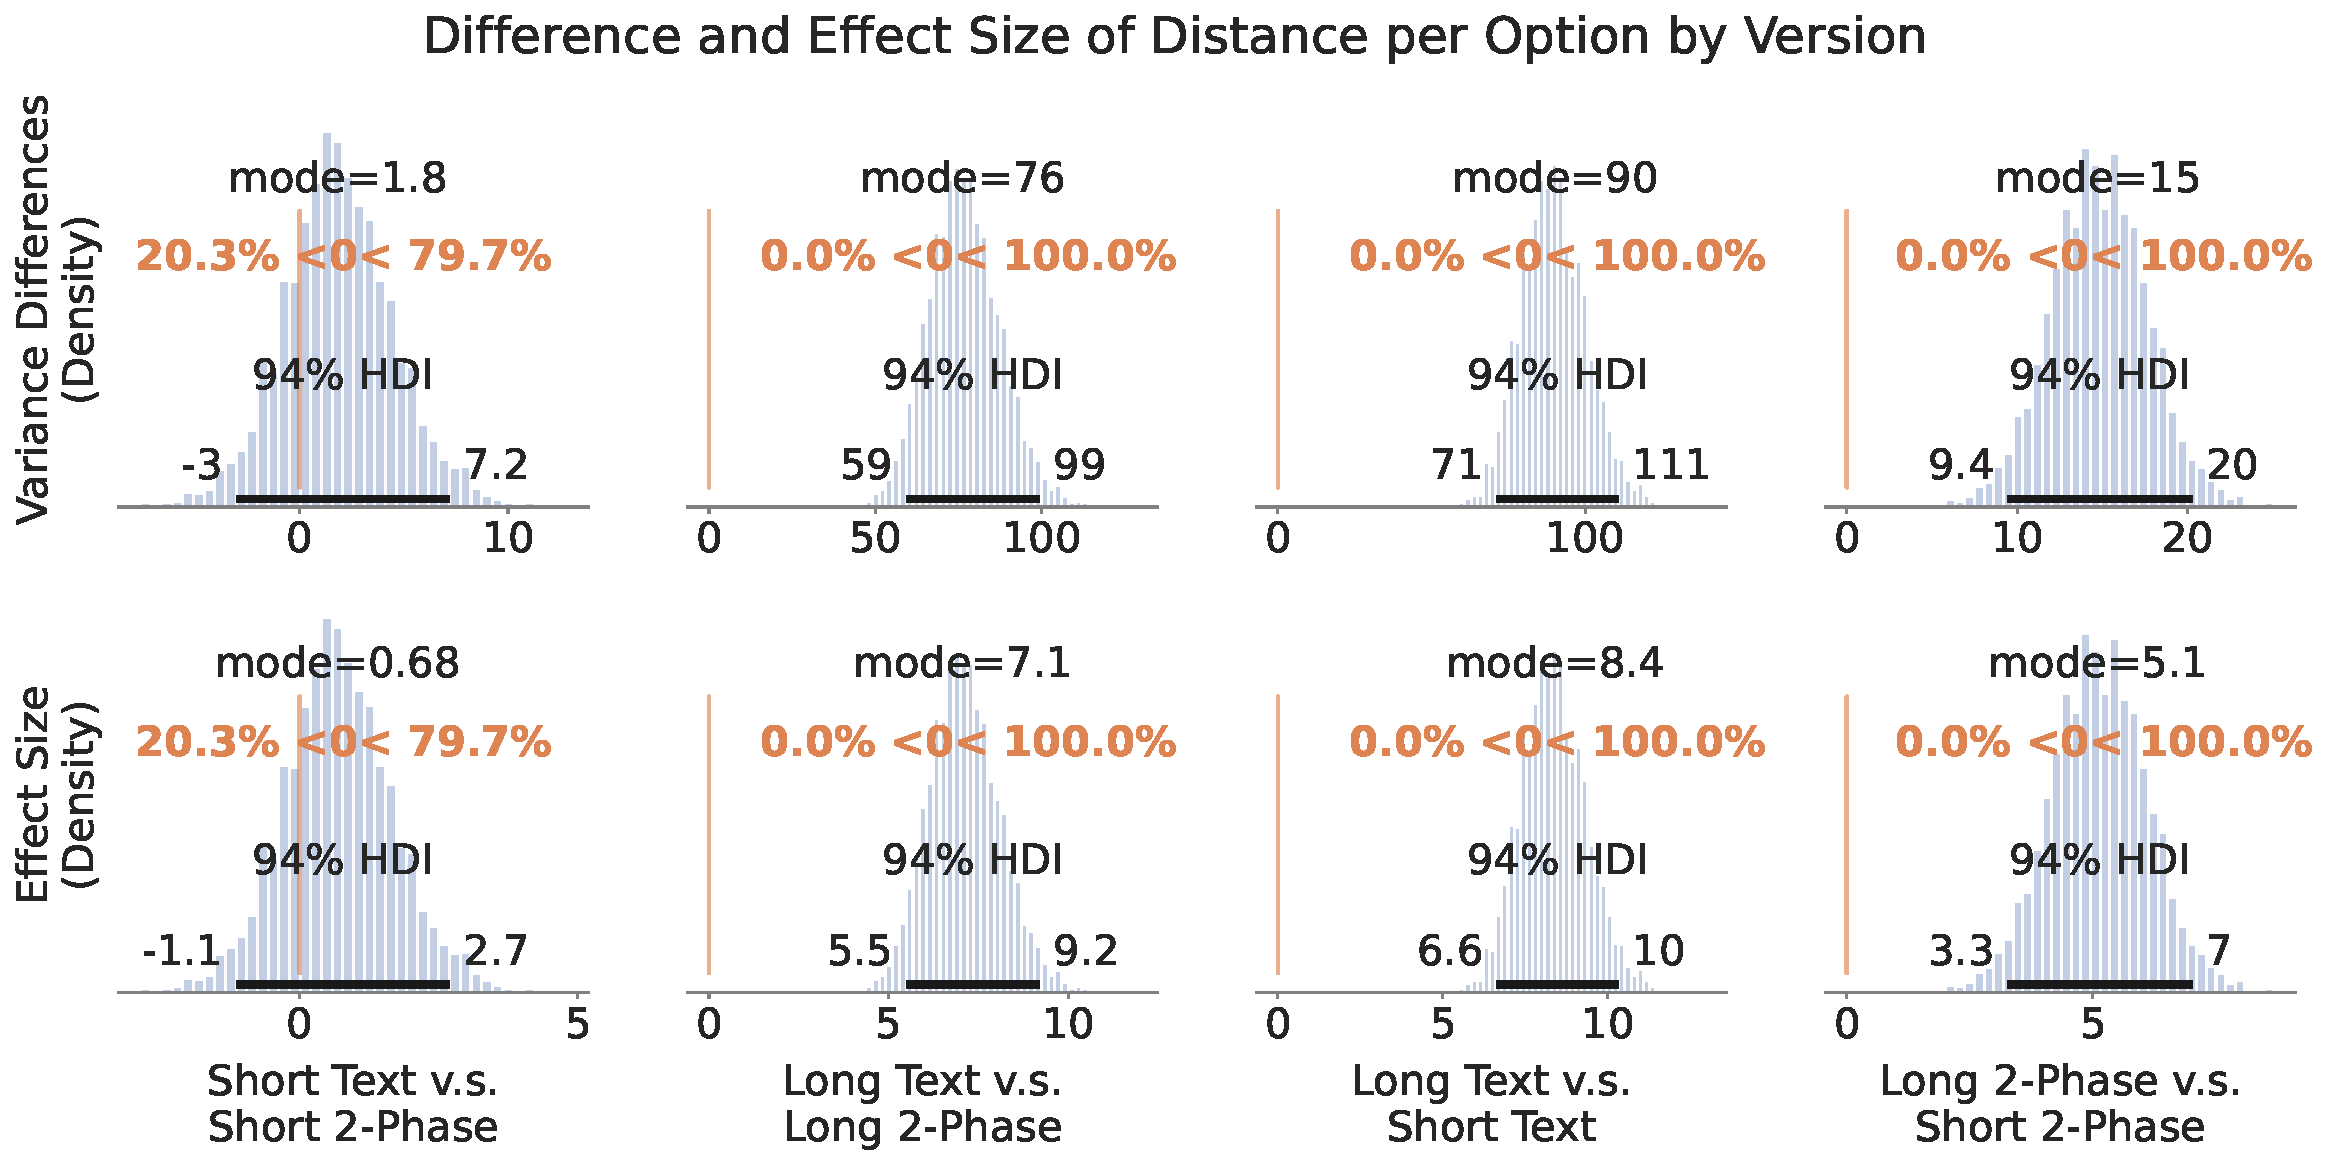
\includegraphics[width=\textwidth]{content/image/distance/distance_diff_per_option_effect_size_by_version_all.pdf}
    \caption{Differences in the variance of edit distance by version.}
    \label{fig:bayesian_distance_variance}
\end{figure}

\subsection{Model 3: Cumulative Edit Distance for long QS} \label{sec:apdx:model_cum_distance}

\subsubsection{Dependent Variables}
The dependent variable for this model is the cumulative edit distance \( D_i \). Cumulative edit distance is a positive continuous variable measured at each step within a version for each user.

\subsubsection{Independent Variables}
The independent variables for this model involve the following. Steps refers to the n-th step when completing QS ($S_i$), and interface version refers to the type of interface used ($V_i$). User-specific effects are also included ($U_{\sigma,i}$). Interface and users are set up with their own hyperpriors.

\subsubsection{Overall Model and Likelihood Function}
We modeled the dependent variable using a **Truncated Normal** distribution (Equation~\ref{eq:model3_likelihood}). The observed outcome variable \( D_i \) represents the response for the \( i \)-th observation parameterized by the latent predictors \( \mu_i \) and \( \sigma_{\text{obs},i} \). The likelihood function is used to model with the intuition that there is a slop and user effect are amplified by steps as described in Equation~\ref{eq:model3_mu}.


\begin{align}
    D_i &\sim \text{TruncatedNormal}(\mu_i, \sigma_{\text{obs},i}, \text{lower}=0) \label{eq:model3_likelihood} \\
    \mu_i &= \alpha_{\text{shared}} + \beta_v[V_i] \cdot S_i + U_i \cdot S_i \label{eq:model3_mu} \\
    U_i &= \mu_{U} + \sigma_{U} \cdot z_{U,i} \label{eq:model3_user_mu}
\end{align}

\subsubsection{Priors}
Priors are defined as:
\begin{align}
    \sigma_{\text{obs},i} &\sim \text{HalfNormal}(0.3) \label{eq:model3_prior_sigma} \\
    \alpha_{\text{shared}} &\sim \mathcal{N}(2.0, 0.5) \label{eq:model3_prior_shared} \\
    \mu_{U}, \sigma_{U} &\sim \mathcal{N}(0, 1), \text{ HalfNormal}(0.1) \label{eq:model3_prior_user} \\
    z_{U,i} &\sim \mathcal{N}(0, 1) \label{eq:model3_prior_z} \\
    \beta_v[V_i] &\sim \mathcal{N}(\mu_{\beta}, \sigma_{\beta}) \label{eq:model3_prior_beta} \\
    \mu_{\beta} &\sim \mathcal{N}(0.05, 0.05) \\
    \sigma_{\beta} &\sim \text{HalfNormal}(0.1) \\
    \sigma_{\phi} &\sim \text{HalfNormal}(0.5) \label{eq:model3_prior_sigma_phi}    
\end{align}

% \begin{align}
%     D_i &\sim \text{TruncatedNormal}(\mu_i, \sigma_{\text{obs},i}, \text{lower}=0) \label{eq:model3_likelihood} \\
%     \mu_i &= \alpha_{\text{shared}} + \beta_v[V_i] \cdot S_i + U_i \cdot S_i \label{eq:model3_mu} \\

    


%     \phi_v[V_i] &= L_{\Omega,\mu} \cdot (\sigma_{\phi,\mu} \odot z_{\phi,\mu}) \label{eq:model3_phi_mean} \\
%     U_i &= \mu_{U,\mu} + \sigma_{U,\mu} \cdot z_{U,\mu,i} \label{eq:model3_user_mu} \\
%     \log(\sigma_{\text{obs},i}) &= \alpha_{\sigma} + \gamma_{\sigma,V_i} + \beta_{I,\sigma}[V_i] \cdot S_i + \phi_{\sigma,V_i} \cdot S_i + U_{\sigma,i} \label{eq:model3_sigma} \\
%     \gamma_{\sigma,V_i} &= \mu_{L,\sigma} + \beta_{L,\sigma} \cdot V_i \label{eq:model3_gamma_sigma} \\
%     \beta_{I,\sigma}[V_i] &= \mu_{I,\sigma} + \sigma_{I,\sigma} \cdot \text{InterfaceEffect}_{\sigma,V_i} \label{eq:model3_beta_I_sigma} \\
%     \phi_{\sigma,V_i} &= L_{\Omega,\sigma} \cdot (\sigma_{\phi,\sigma} \odot z_{\phi,\sigma}) \label{eq:model3_phi_sigma} \\
%     U_{\sigma,i} &= \mu_{U,\sigma} + \sigma_{U,\sigma} \cdot z_{U,\sigma,i} \label{eq:model3_user_sigma}
% \end{align}

% \subsubsection{Priors}
% Priors are defined as:
% \begin{align}
%     \mu_{\text{shared}}, \alpha_{\sigma} &\sim \mathcal{N}(0, 1) \label{eq:model3_prior_shared} \\
%     \mu_{L,\mu}, \mu_{I,\mu}, \mu_{U,\mu}, \beta_{L,\mu}, \beta_{I,\mu}, z_{\phi,\mu}, z_{U,\mu,i} &\sim \mathcal{N}(0, 1) \label{eq:model3_prior_mean} \\
%     \mu_{L,\sigma}, \mu_{I,\sigma}, \mu_{U,\sigma}, \beta_{L,\sigma}, \beta_{I,\sigma}, z_{\phi,\sigma}, z_{U,\sigma,i} &\sim \mathcal{N}(0, 1) \label{eq:model3_prior_variance} \\
%     \sigma_{\phi,\mu}, \sigma_{\phi,\sigma} &\sim \text{HalfNormal}(0.5) \label{eq:model3_prior_sigma_phi} \\
%     \sigma_{U,\mu}, \sigma_{U,\sigma} &\sim \text{Exponential}(0.5) \label{eq:model3_prior_sigma_U} \\
%     L_{\Omega,\mu}, L_{\Omega,\sigma} &\sim \text{LKJ}(3) \label{eq:model3_prior_L_Omega}
% \end{align}